
% Operations Manual Title
\infolevone{
\section{Compton Polarimeter}
%\setcounter{subsection}{0}

The Compton Polarimeter provides a continuous, non-destructive measurement of the electron
beam polarization. The system was installed and commissioned in 2010 and has been updated
for use at 11~GeV. The Compton polarimeter is located in the Hall C alcove, just upstream of
the M\o ller Polarimeter (between the 3C19 and 3C20 girders). Accelerator Operations
sets up beam through the Hall C Compton chicane as part of the Hall C Beam Delivery Procedure:
\newline
\htmladdnormallink{opsntsrv.acc.jlab.org/ops\_docs/MCC\_web\_interface/interface\_pages/operating\_procedures.asp}{opsntsrv.acc.jlab.org/ops\_docs/MCC\_web\_interface/interface\_pages/operating\_procedures.asp}

An overview of the Compton Polarimeter is shown in Fig.~\ref{fig:compton_overview}. The main components
of the Compton Polarimeter are:

\begin{enumerate}
 \item{A 4--dipole chicane that deflects the beam vertically (down) by 13~cm where it interacts
 with a laser system and is then steered back to the nominal beam height.}
 \item{A laser system in which a 10~W CW laser is coupled to a moderate gain Fabry-P\'{e}rot
 cavity which results in up to 2~kW of stored laser power.}
 \item{A compact photon detector consisting of a 4 crystal lead-tungstate array read out by a single
 photomultiplier tube.}
 \item{A highly segmented, diamond strip electron detector for detecting the Compton scattered electrons.}
\end{enumerate}

\begin{figure}[htp]
\begin{center}
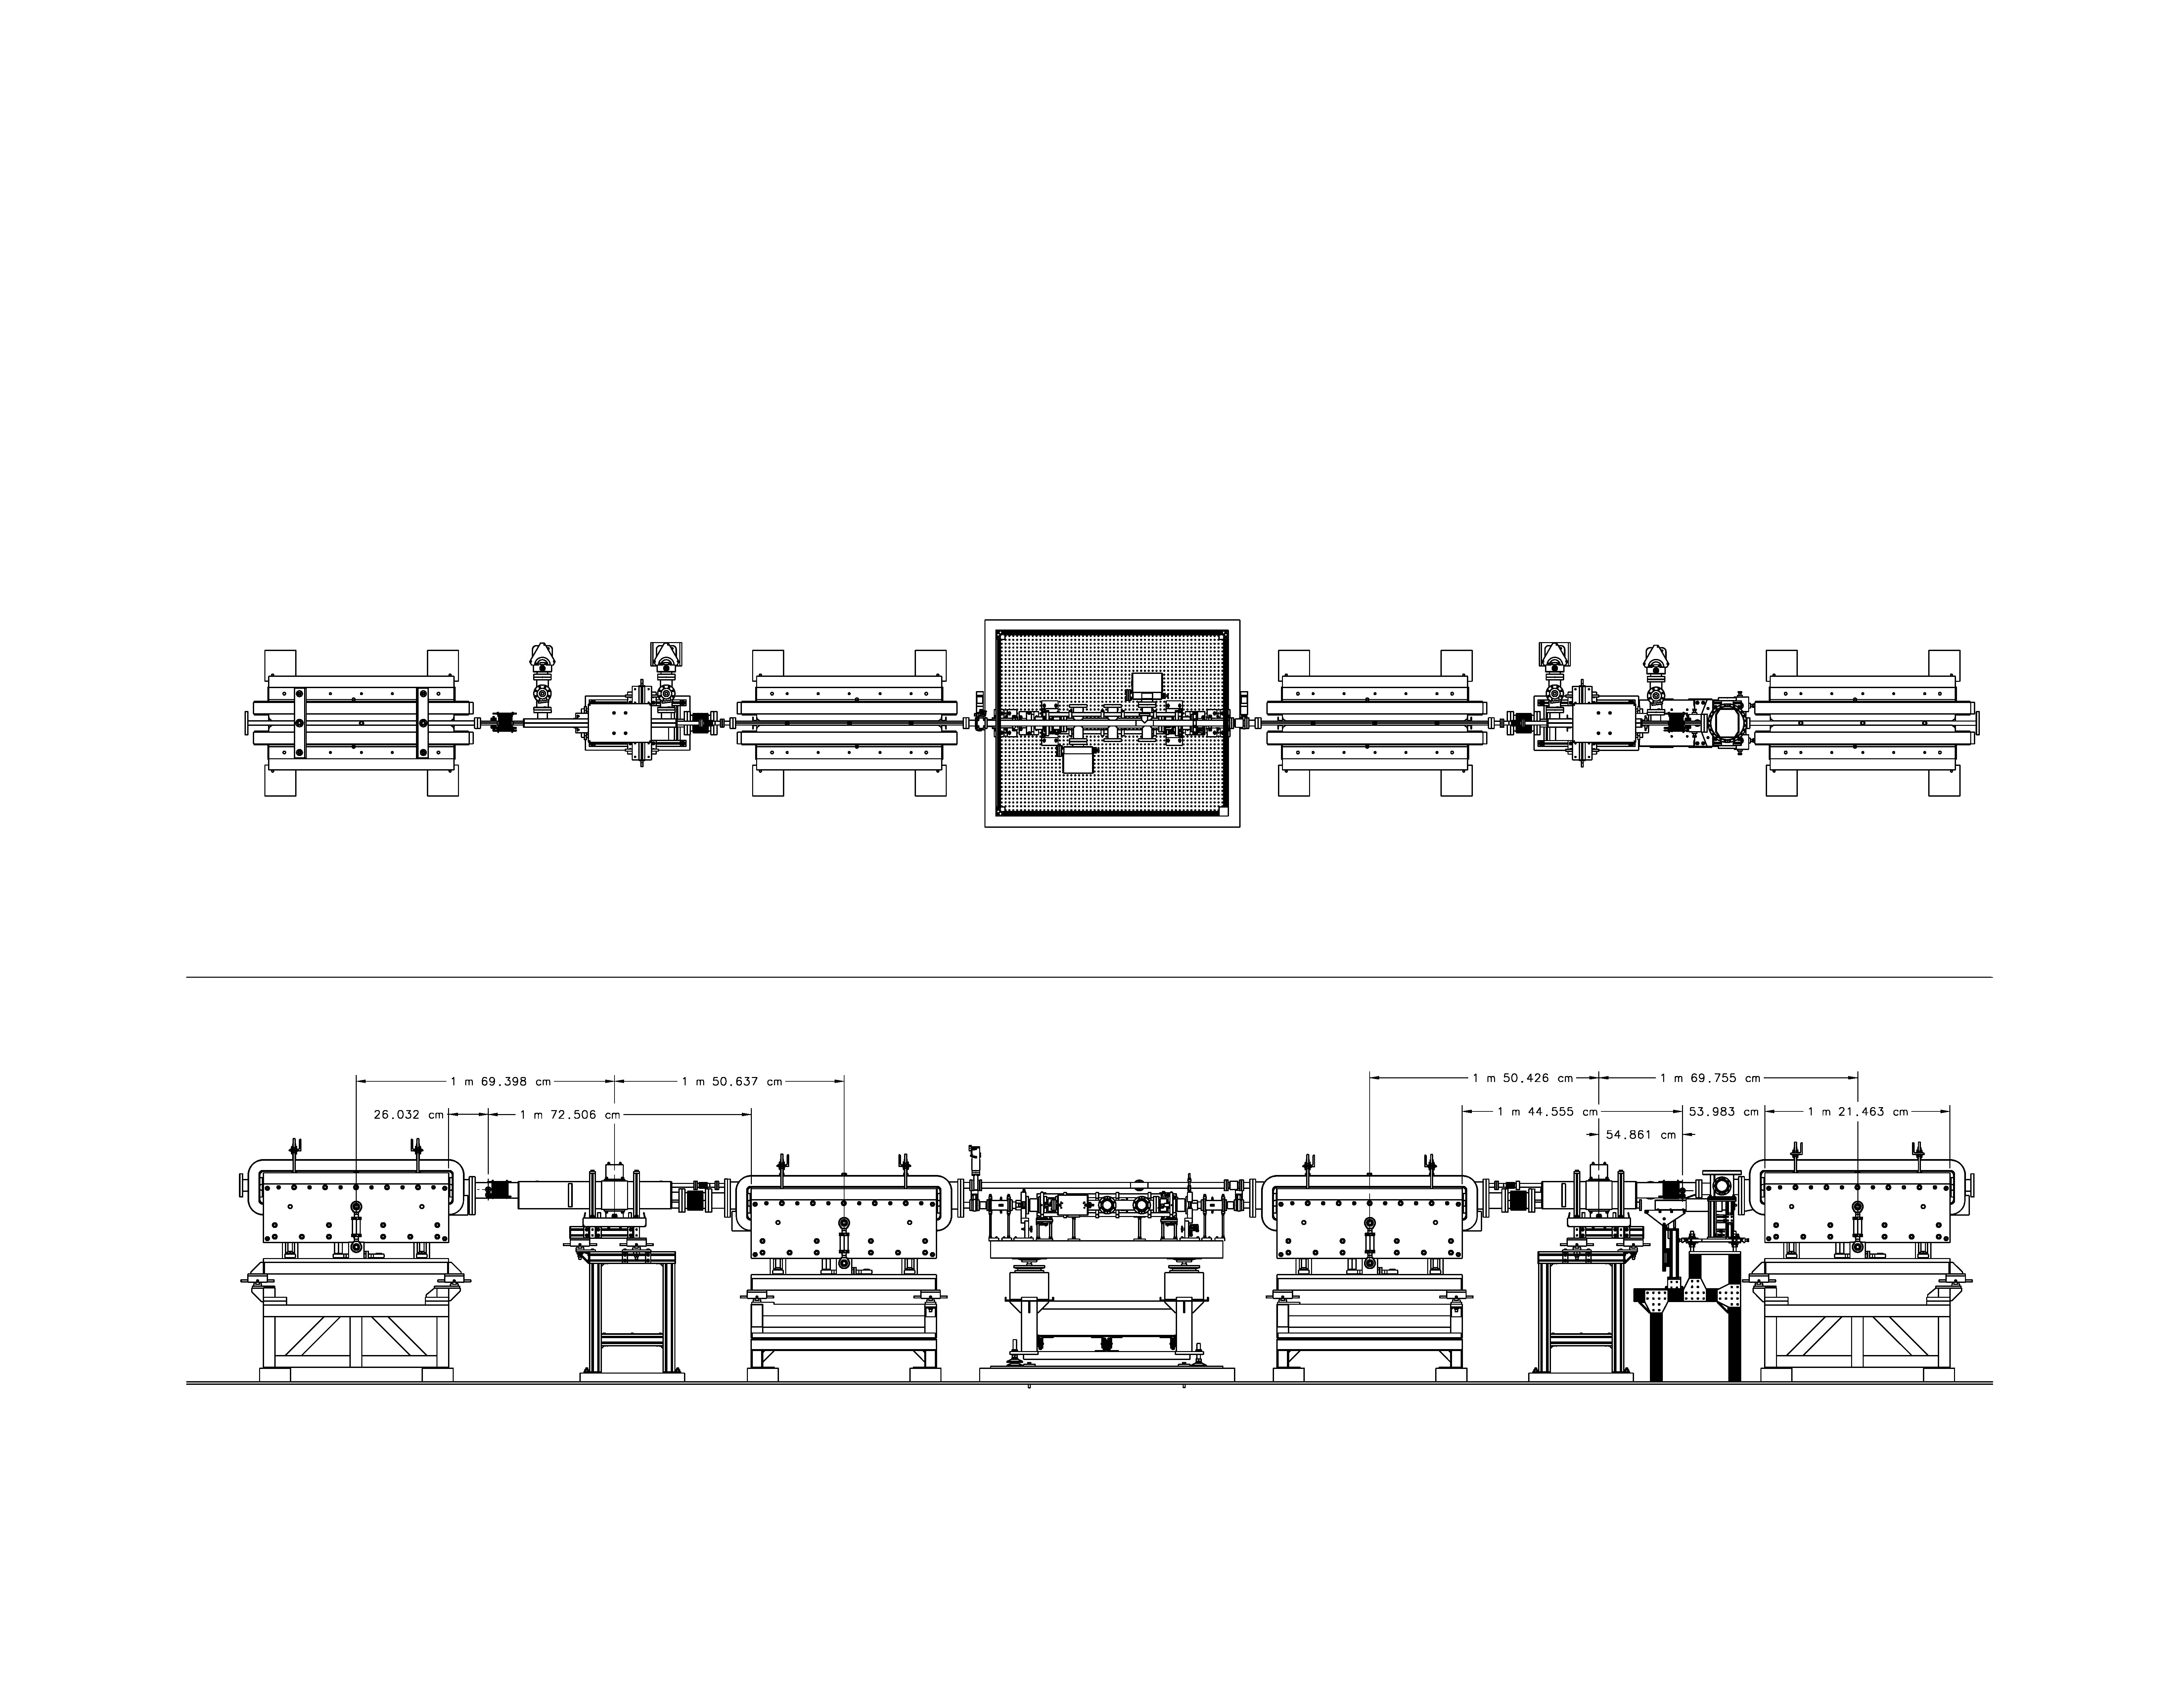
\includegraphics[width=15cm]{COMPTON_JAY_LAYOUT.pdf}
\caption{Overview of the Compton polarimeter in Hall C.\label{fig:compton_overview}}
\end{center}
\end{figure}

\subsection{Polarimeter Description}
The Hall C Compton polarimeter is used to make continuous, non-destructive measurements of the beam
polarization using the well--understood electron-photon (Compton) scattering process. Due to the relatively
low luminosity of the Compton scattering process, the Compton polarimeter can be used without impacting
the data-taking of the main experiment.

The Compton polarimeter works as follows. The electron beam is steered from its nominal height to a laser
system which sits 13~cm below beam height. The electron beam collides with 2.3~eV photons provided by a
high power laser system. The high power laser system consists of a resonating Fabry-P\'{e}rot cavity, locked
to a CW, 10~W laser. After collision, the laser-photon is boosted backwards and has maximum energies ranging
from 45~MeV (for 1~GeV beam energy) to 3~GeV (for 11~GeV beam energy).  The backscattered photons
are detected in a compact, lead-tungstate detector. This detector operates in ``energy-integrating'' mode, measuring
the asymmetry in the total energy deposited for each electron beam helicity state. The beam electrons also lose
energy in the Compton scattering process. These electrons will be deflected away from the unscattered electrons
as they pass through a dipole downstream of the interaction region. The scattered electrons are detected
in the segmented, diamond-strip electron detector.  The electron detector must be movable, since the scattered
electrons' separation from the beam will change with beam energy. In principle, the electron detector can
function at distances as close as 5~mm from the beam.

The photon and electron detectors provide quasi-independent measurements of the electron beam polarization;
while the detector systematics are very different, they do share common systematic uncertainties from the laser
system.

\subsubsection{Dipole chicane}
The Compton polarimeter chicane allows the electron beam to be deflected 13 cm from its nominal beam
height to interact with the laser system between dipoles 2 and 3, allow detection of the backscattered
photon, and provide momentum analysis of the scattered electron. The overall length of the chicane is about
11.1 meters (entrance of dipole 1 to exit of dipole 4). The distance between dipoles 1-2 and 3-4 is 1.95~m,
with 2.2~m allocated for the interaction region between dipoles 2 and 3.

The key components of the chicane are four identical dipoles of length 1.25~m. The dipoles were
designed by MIT-Bates and manufactured by Buckley Systems. Nominal properties of the dipoles are listed
in Table~\ref{tab:compton_dipoles} and a photograph is shown in Fig.~\ref{fig:magnet_photos}. The four
dipoles are connected in series and powered from a single power supply. A few turns in the coils of the
dipoles are controlled separately by low power supplies (trim cards) to allow $\approx$2\% independent variation
of the strength of each dipole.

\begin{table}[hbt]
\begin{center}
\begin{tabular}{|l|l|} \hline
Bend angle        &   2.3$^{\circ}$ \\
Field at 11 GeV   &   12.5 kG \\
Effective length  &   1.246 m \\
Max. current      &   250 A  \\
Turns/coil        &  64 \\
Resistance @ 25$^\circ$ C & 75 m-Ohms \\
Coil voltage      & 20 V x 2 \\
Weight            & 275 lbs./coil \\
                  & Steel=5000 lbs. \\
\hline
\end{tabular}
\caption{Compton dipole properties.\label{tab:compton_dipoles}}
\end{center}
\end{table}


While the trim coils allow vertical correction of the orbit through the chicane, correctors between
dipoles 1-2 and 3-4 allow horizontal beam adjustment. Because of the large vacuum chambers required
between the Compton dipoles, the horizontal correctors encompass both the ``straight-through'' and
``chicane'' beam paths. The large size of the correctors also lead to larger than usual stray fields -
these are mitigated using a magnetic shield mounted over the corrector coils. A photograph of the horizontal
corrector is shown in Fig.~\ref{fig:magnet_photos}.

\begin{figure}
\begin{center}
\subfloat[Compton polarimeter dipole]{\includegraphics[width=0.7\linewidth]{compton_12GeV_poles.png}}\\
\subfloat[Compton horizontal corrector]{\includegraphics[width=0.5\linewidth]{compton_corrector.png}}
\caption{Photographs of magnets used in the Compton chicane. The top picture shows one of
the Compton dipoles (mounted for field measurement). The bottom picture shows one of the new, large
horizontal correctors mounted on its stand. The magnetic shield (not yet installed in this picture) can be
seen on the floor next to the corrector stand.\label{fig:magnet_photos}}
\end{center}
\end{figure}

In addition to the magnetic components of the Compton chicane, beam diagnostics are used to ensure the
correct orbit of the beam through the chicane and to minimize the chances of damage to detector components.
Two standard beam position monitors are located on the upstream and downstream ends of the laser table. These
are used to provide knowledge of the beam trajectory where it collides with the laser and are used
as part of a slow position lock. In addition, BPMs are used between dipoles 1-2 and 3-4 to provide knowledge
of the beam position as it exits dipole 1 and enters dipole 4. Because of the limited space available,
these BPMs are not standard stripline BPMs, but rather are so-called ``button'' style BPMs, mounted
directly in the vacuum chamber. Typically, an ion chamber is also placed near the electron  detector
to minimize the chance of beam excursions damaging the diamond strip detector. Two small scintillators
are also placed on the laser table, right next to the beam pipe to help monitor beam-related backgrounds
near the laser. These detector are provided and maintained by Hall C, but the EPICS signals showing the rates
from these detectors are provided to the accelerator operators.


\subsubsection{Laser system}
The Compton laser system consists of a moderate gain ($\approx$200) Fabry-P\'{e}rot cavity, pumped by a 10 W
CW green laser (Coherent Verdi V10). In order to store power in the cavity, the length of the cavity must
equal an integer number of laser wavelengths ($L_{\textrm{cavity}}=n\lambda$). This is achieved by feeding back
on the laser wavelength via the so-called Pound-Drever-Hall (PDH) technique. The wavelength modulation
of the Verdi laser is achieved via PZT stacks that adjust the lasing cavity length inside the laser head.

The laser system sits on a small optical table (with pneumatic vibration-isolating legs) between
dipoles 2 and 3. During normal operation, an interlocked cover prevents any laser light from leaving
the optical table. In addition, laser safety curtains surround the laser table. During alignment of
the laser and optical elements, additional laser safety curtains are dropped creating a mini-laser room.
While the alignment is ongoing and the laser table cover is removed, pressure sensitive floor mats prevent
accidental ``walk-through'' of the laser area. The safety interlock system and its features are fully
described in the Hall C Compton Laser Safety Operating Procedure (LSOP). 

The main components of the laser system are:
\begin{enumerate}
 \item{The 10~W, Coherent Verdi V10 laser. This laser has been modified to include two PZT stacks for slow and
 fast wavelength adjustment of the laser.}
 \item{Optics for laser beam steering, shaping, and polarization control.}
 \item{Optical detectors for monitoring incident and transmitted laser power, laser beam position, and for
 use with the PDH feedback system.}
 \item{Moderate gain Fabry-P\'{e}rot cavity. The low-loss cavity mirrors live inside the beamline vacuum and
 have a nominal reflectivity of 99.5\% with losses better than 50 ppm.}
 \item{Feedback electronics for matching the laser wavelength to the Fabry-P\'{e}rot cavity length. The
 Hall C Compton polarimeter uses a commercial FPGA-based module manufactured by Toptica Photonics called the
 Digilock-110.}
 \item{Slow controls system. We use remotely controllable (closed-loop) mirror mounts and rotation stages
 manufactured by New Focus for controlling the laser beam steering and polarization on the table. The control
 system is written in LabView and runs on a PC that is located just inside the labyrinth that leads to Hall C.
 The slow control system allows remote control of the Verdi laser, the New Focus optics stages, and interfaces
 with the Digilock locking electronics to allow automated locking and unlocking of the cavity.}
 \end{enumerate}

A detailed schematic of the layout of optical components on the laser table is shown in
Fig.~\ref{fig:laser_table}.  To summarize briefly: The laser is positioned on the downstream, beam left
corner of the table. The polarization controlling optics are on the other side of the table. The laser
is brought from ~2 inches above table height up to beam height via a periscope. The laser enters the vacuum
pipe from the beam right side and is steered into the cavity from downstream. The transmitted laser beam
(upstream of the cavity) exits from bottom of the vacuum pipe and is steered to power monitoring detectors
as well as a CCD camera.


\begin{figure}[htp]
\begin{center}
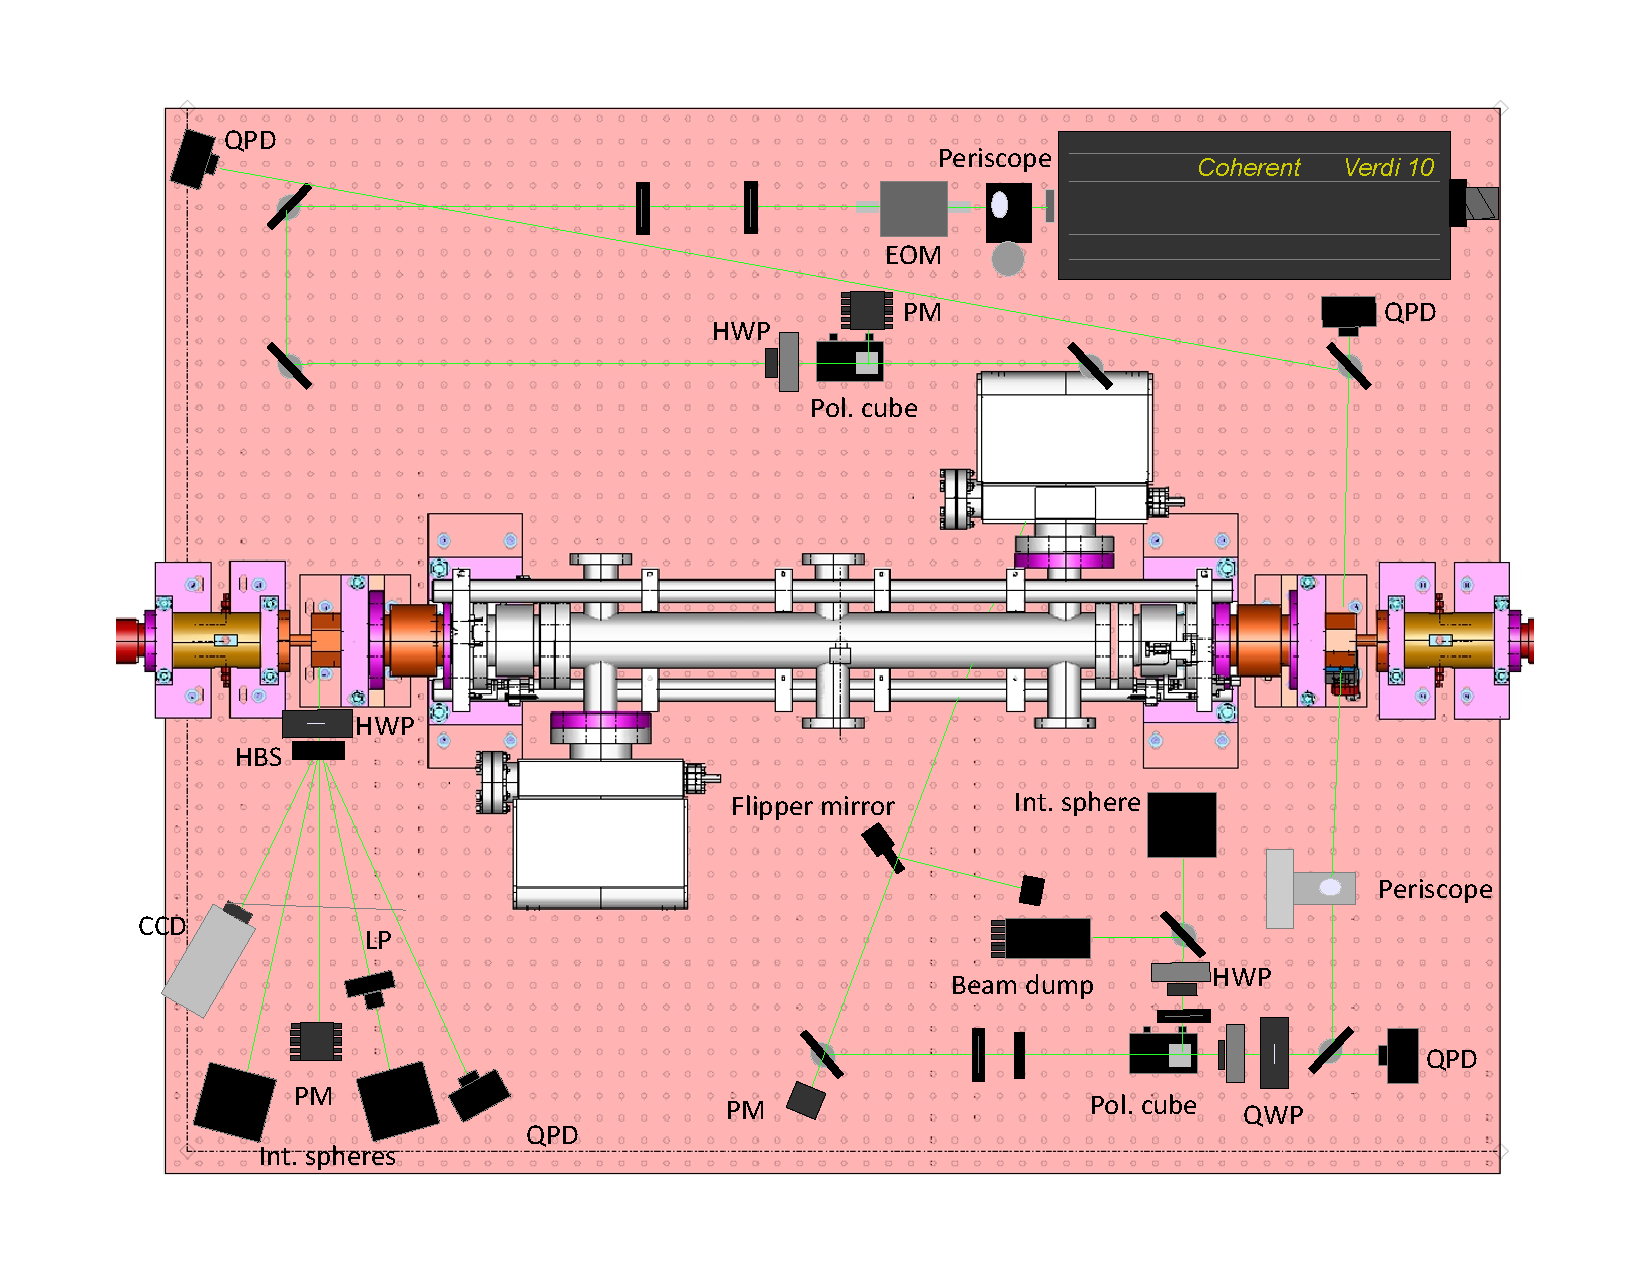
\includegraphics[width=15cm]{hallc_compton_tablelayout_2013.pdf}
\caption{Laser table layout for Hall C Compton polarimeter. The output of the Verdi goes through a
variety of optics used for intensity control, frequency modulation, and mode-matching before
entering the low gain Fabry-P\'{e}rot cavity. Upon exiting the cavity, the power and polarization of the
laser is monitored on the “analysis” station. Key: EOM = electro-optic modulator, HWP=half-wave plate,
QWP=quarter-wave plate, PM=power meter, QPD=quad-photodiode, HBS=harmonic beam sampler.
\label{fig:laser_table}}
\end{center}
\end{figure}

As noted earlier, the laser is controlled via a LabView program running on a PC in Hall C. The controls
can be accessed by a Compton laser expert using a VNC session from the Counting House.  The laser slow
controls are never accessed by a non-expert: only Compton laser experts are authorized to manipulate the
system. The LabView control program does interface with EPICS, but only for the purpose of providing
readback and archiving of laser-related quantities.  No features of the laser system can be modified
from EPICS.

The LabView control program incorporates several ``tabs'' to manipulate various aspects of the system. These
tabs include:
\begin{enumerate}
 \item{Optics control: steering of the laser into the cavity and visualization of the laser position via
 position sensitive detectors (QPDs).}
 \item{QPD readout: manipulation and diagnostics of the QPD readout loops.}
 \item{Laser controls: control of the Coherent Verdi V10 laser.}
 \item{Digilock: readback of the parameters used in the cavity feedback electronics as well as control
 of the lock and unlocking intervals. This tab is not typically used to control the Digilock directly. Rather
 that is done using a control program provided by the manufacturer of the Digilock module.}
 \item{Transfer function: used for measurements required for constraining the degree of polarization inside the
 cavity. These measurements are not typically done during ``production'' running.}
 \item{Polarization: setup of the laser polarization via manipulation of the rotation stages that hold
 half and quarter wave plates.}
 \end{enumerate}

Fig.~\ref{fig:laser_controls} shows the LabView laser system controls, with the top plot showing the
``Optics Control'' tab and the bottom plot showing the ``Feedback Controls'' tab.


\begin{figure}[htp]
\begin{center}
\subfloat[Mirror/steering controls]{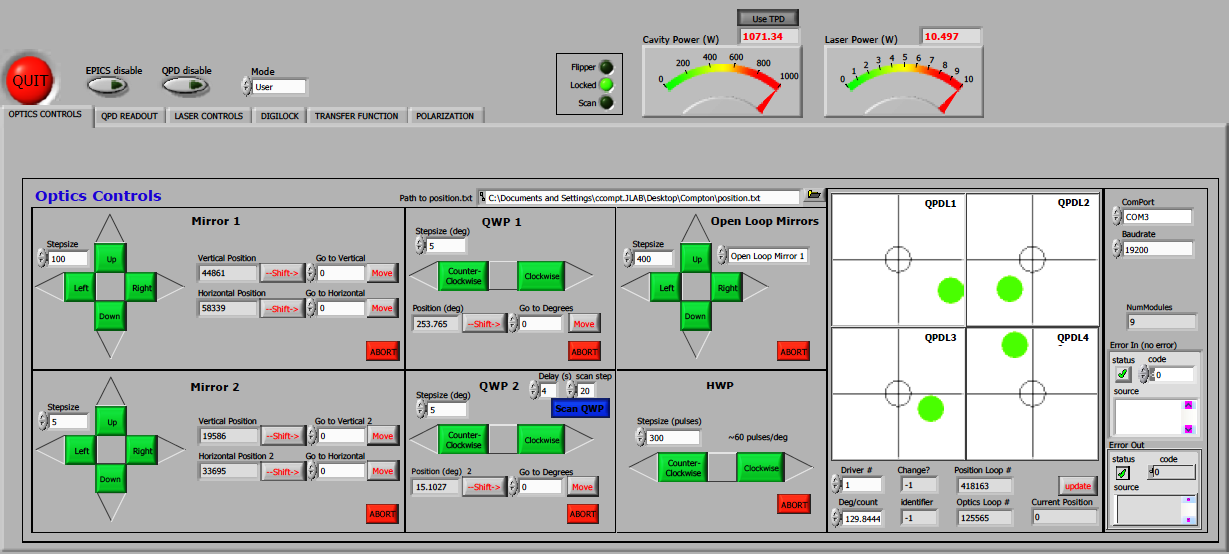
\includegraphics[width=15cm]{opticsloop.png}}\\
\subfloat[Feedback controls]{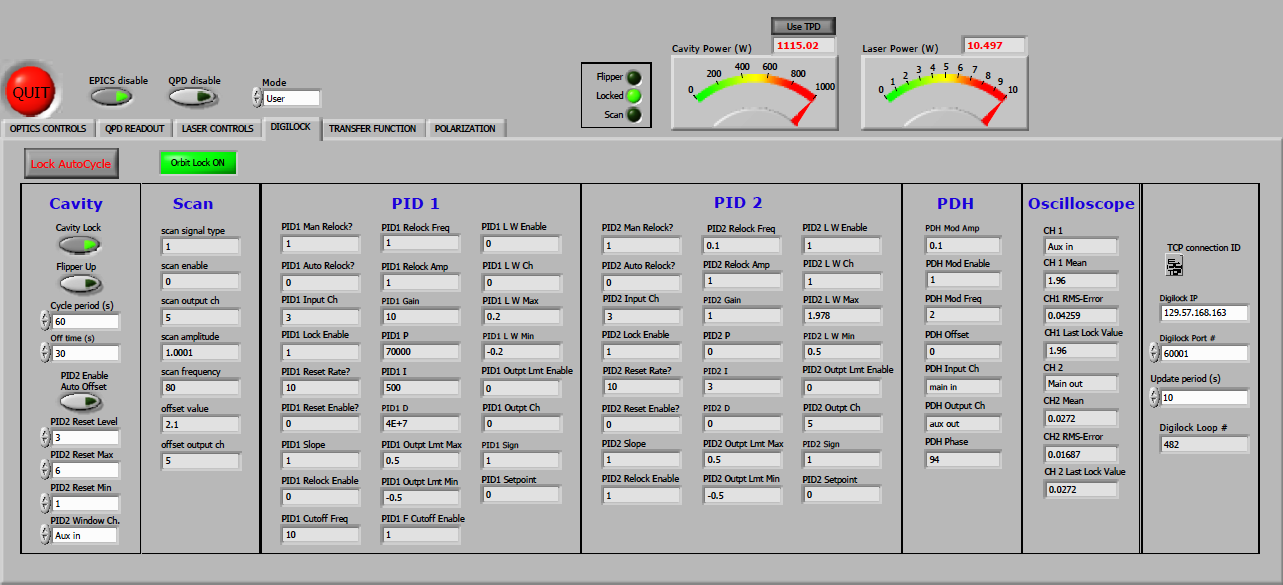
\includegraphics[width=15cm]{dgkloop.png}}
\caption{Slow controls for the Compton laser system.  The top panel shows the controls for the
two steering mirrors located just before the laser enters the beamline vacuum. The bottom panel
shows the readback of variables set in the commercial locking module and allows control of the time
scales for locking and unlocking the cavity.\label{fig:laser_controls}}
\end{center}
\end{figure}


\subsubsection{Electron Detector}
The electron detector in use is a 21mm x 21mm CVD diamond microstrip. Four planes are used in coincidence with
each of the 4 planes separated by 1cm with the strips of each plane aligned to $\approx$20~$\mu$m. Each plane contains
96 horizontal diamond strips (polycrystalline CVD diamond). Each strip is 180~$\mu$m wide with a 20~$\mu$m gap
separating each strip. Metalization was done on each plane with Titanium-Platinum-Gold (TiPtAu). The
carrier boards are Ceramic (alumina).  A single plane of the electron detector is shown in
Fig.~\ref{fig:edet_photo} with a detailed schematic in Fig.~\ref{fig:edet_schematic}.

The strips are connected to custom, low-noise amplifier discriminator boards (Q-Weak Amplifier
Discriminators, QWADs) via 55~cm long, Kapton flexible circuit boards with capacitance 60-90~pF. Each QWAD
has 48 channels, thus requiring 2 QWAD boards per plane. One QWAD processes the signal from all odd strips
of the detector, while another processes the signals from all even strips.

The QWAD can accept signals of both positive and negative polarity with a jumper on the board setting the
appropriate configuration (the electron detector operates at negative polarity).  The QWAD utilizes 3
different power supplies. For the main power input, we use two Acopian 5 V supplies to provide positive and
negative 5~V. These supplies are behind the green wall near the entrance to Hall C in rack HC01Z02. 

Agilent 3633A power supplies (also located in Hall C, neat the Acopian supplies) are used for setting the
external threshold of the QWAD. In the usual operating mode it can deliver a maximum output of 8.0 V.
The Agilent power supply used for external threshold can be remotely accessed via port 11 on hall C
terminal server 5. One can access this by the command from any cdaq machine:
\begin{itemize}
\item{Type \texttt{telnet hctsv5 2011}}
\item{Next, access the telnet prompt by pressing \texttt{Ctrl + ]}}
\item{At the telnet prompt explicitly set the line mode on the terminal: \texttt{telnet> mode line}}
\end{itemize}


\begin{figure}[htp]
\begin{center}
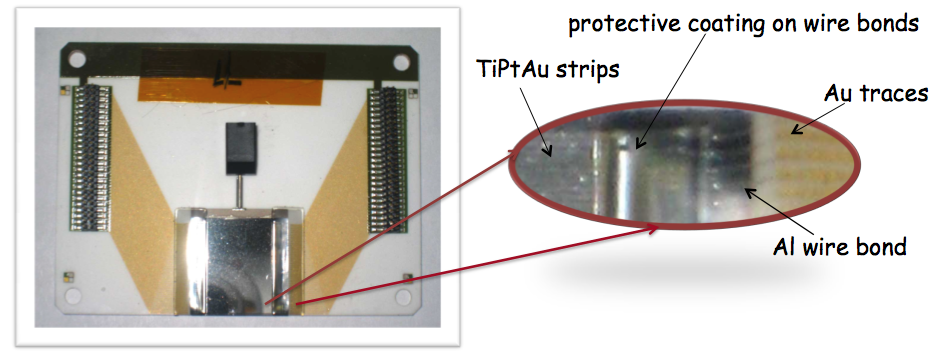
\includegraphics[angle=0,width=15cm]{El_det_diamond.png}
\caption{Picture of one of the diamond strip detector planes.\label{fig:edet_photo}}
\end{center}
\end{figure}

\begin{figure}[htp]
\begin{center}
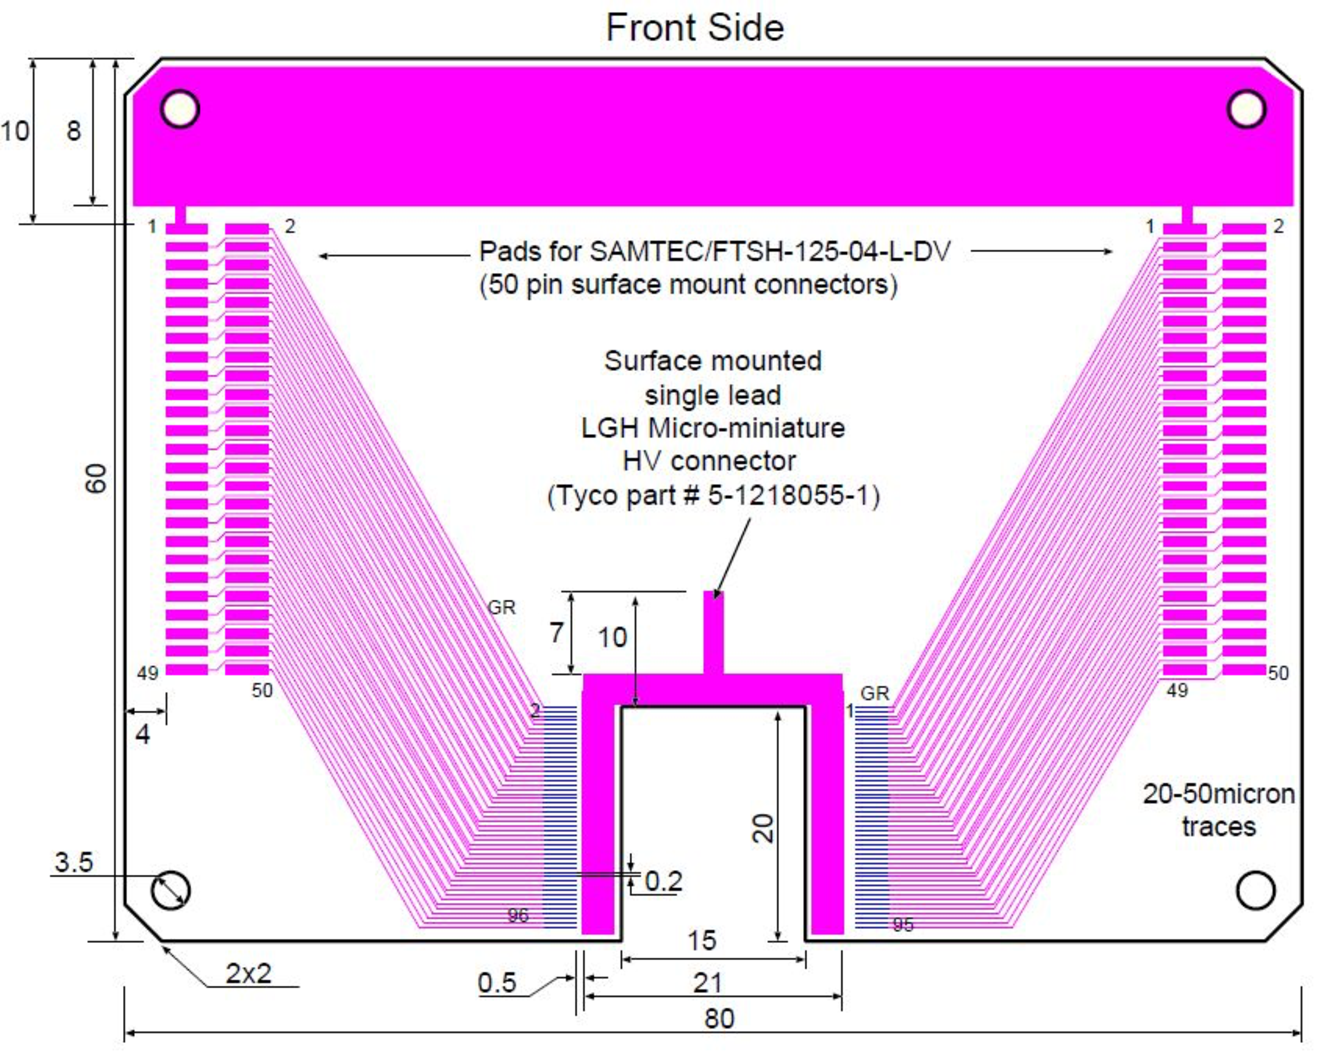
\includegraphics[angle=0,width=7cm]{EDet_front_schematic.pdf}
\caption{Detailed schematic of diamond detector plane.\label{fig:edet_schematic}}
\end{center}
\end{figure}

We use an NHQ 202L HV power supply to give HV to the diamond micro strip detectors. The detectors are
typically operated at -400~V. The module is set to deliver negative voltage through a turn-switch on its side
(not visible on the front panel). The actual value of the voltage can be set by the front panel knob or
remotely. If the module is intended to be operated remotely. the DAC flip-switch should be flipped away from
the knob. The high voltage module is located in a NIM bin in the Compton racks in the Hall C Counting House.
A standard SHV cable runs from the module to a feed-through located at the top the electron detector
vacuum can. The HV module is connected to port server hctsv4 at port 3. In order to connect to the device
once has to execute from any cdaqlX terminal, \texttt{telnet hctsv4 2003}.

The Compton electron detector can be moved vertically to allow the detector to be placed totally out of beam,
or moved into position for a Compton measurement. The detector motion is accomplished using an MDC 665529
linear motion stage (with an 8 inch full range of motion) with stepper motor, controlled by an IDC S6961
motion controller.  The motion control program is hosted on iochc10 (located in Hall C, also used for
M\o ller polarimeter slow controls) and the control interface is via EDM.

It is important to note that the Hall C Compton electron detector is interfaced with the accelerator
fast-shutdown (FSD) system. If the Compton dipole chicane is not energized (i.e. dipole power supply is off),
the electron detector must be in its fully retracted position (indicated via a limit switch) to allow
beam delivery. Only if the chicane is energized, can the detector be moved away from its fully out
position. In addition, if the detector moves while beam is on, an FSD will be triggered.

The Compton electron detector motion program can be started as follows:
\begin{enumerate}
    \item{Log in to any cdaqlX as \texttt{cvxwrks}.}
    \item{\texttt{cd MEDM/compton}}
    \item{\texttt{edm -x HLC\_E\_CompED.edl }}
\end{enumerate}
The electron control GUI is shown in Fig.~\ref{fig:edet_motion_gui}.


\begin{figure}[htb]
\begin{center}
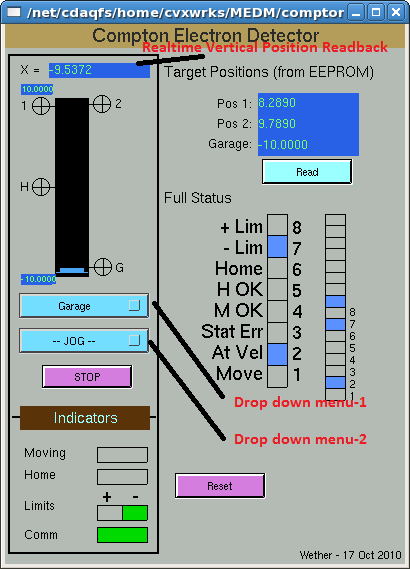
\includegraphics[angle=0,width=7cm]{Edet_parked.png}
\caption{Compton electron detector motion GUI. In this picture, the detector is fully out of beam,
indicated by the activation of the ``-'' limit switch.\label{fig:edet_motion_gui}}
\end{center}
\end{figure}

Before any motion on the e-detector is attempted, call MCC beam to request beam OFF and mask the Compton
electron detector motion FSD. There is no visual verification of this FSD on the motion GUI, so please
confirm the masking before moving the detector.

The electron detector motion GUI has several pre-defined positions selectable from the drop-down menu.
``Garage'' removes the detector from beam. ``Pos 1'' and ``Pos 2'' are two positions manually programmed
into the controller to be close to the nominal electron detector running position. One can also ``jog'' the
detector using a set of pre-defined, small increments (0.1 to 0.5 cm steps).


\subsubsection{Photon Detector}
The Compton polarimeter photon detector is used to detect the backscattered photons from the Compton
scattering process. The photon detector is located at the same height as the laser--electron beam interaction
(i.e., centered at 13 cm below nominal beam height). The detector sits downstream of the third dipole,
just upstream of the electron detector. The backscattered photons travel through the vacuum chamber of dipole~3,
into the vacuum chamber between dipoles 3-4 and exits through a 0.5~mm thick window (radius 1.74 cm).

The detector itself consists of 4 lead-tungstate crystals; each crystal is 3 x 3 cm wide, 20~cm long. The inner
surfaces of the crystals are in optical contact (not individually wrapped) and the light from the crystals is
detected in a single 3--inch PMT (Hamamatsu H6526 PMT+base assembly).  The detector typically runs at
$\approx$-1700~V, provided from a HV supply in the Hall C Counting House. The PMT signal is also sent to the Counting
House where it is read out in a flash ADC.

In addition to the detector itself, an LED system is used for gain monitoring. This system consists of 2 LEDs flashing
at different rates and strengths to provide relative monitoring of the system gain and stability. The LEDs sit in
small boxes below the detector and are connected via optical fiber to the detector itself. No hazards are associated
with these LEDs due to the low voltages used to drive them and the diffuse, low--power of the light emitted.

%\subsection{Compton Setup Procedure}


\begin{safetyen}{0}{0}
\infolevone{\subsection{Safety Information}}
%
% Information for the ESAD
%

The Compton Polarimeter integrates beamline elements (magnets and vacuum systems) with
particle detector systems. Typical hazards for both types of systems are present.

\infolevone{\subsubsection{Hazards}}
\infoleveqnull{\subsection{Hazards}}

There are several specific hazards (potentially beyond those found in the accelerator beamline)
associated with the Compton Polarimeter.  These include:
\begin{enumerate}
\item{Laser hazards: A high power laser system is contained between the 2nd and 3rd dipoles in the polarimeter chicane.}
\item{Electrical hazards: These exist in the vicinity of the magnet leads, as well as the detector high
voltage.}
\item{Magnetic fields from the dipole magnets and new horizontal corrector magnets.}
\end{enumerate}

\infolevone{\subsubsection{Mitigations}}
\infoleveqnull{\subsection{Mitigations}}

The special hazards associated with the Hall C Compton are mitigated as
described below.

\begin{enumerate}
  \item{Laser hazards for the non-expert are mitigated by signage, flashing beacons to indicate the laser is
  on, and the containment of the laser system in on a fully-enclosed and interlocked laser table. Any
  attempt to access the laser area will result in automated shut-down of the laser. The Hall C Compton
  laser system safety procedures are fully described in the Laser Safety Operating Procedure (LSOP).}
  \item{Electrical hazards due to magnet leads are mitigated using shields or covers over magnet leads where
   appropriate.  The Compton detectors (outside the beamline vacuum) use standard SHV connectors. The electron
   detector planes use a mini-HV connector mounted to the plane - however, these are not accessible during
   normal operation.}
  \item{``Magnet on'' signs or blinking lights alert users to the presence of magnetic fields. The new
  horizontal corrector magnets between dipoles 1-2 and 3-4 also have additional magnetic shielding to mitigate the
  presence of any stray field.}
\end{enumerate}

\noindent{}Additional safety information is available in the following documents:
\begin{list}{--}{\setlength{\itemsep}{-0.15cm}}
  \item EH\&S Manual~\cite{EHScebaf};
  \item PSS Description Document~\cite{PSScebaf}
  \item Accelerator Operations Directive~\cite{AODcebaf};
\end{list}

\infolevone{\subsubsection{Responsible Personnel}}
\infoleveqnull{\subsection{Responsible Personnel}}

Points of contact for the Hall C Compton Polarimeter are listed in the Tab.~\ref{tab:personnel_compton}.

\begin{namestab}{tab:personnel_compton}{Compton Polarimeter: authorized personnel}{%
   Compton Polarimeter points of contact.}
  \DaveGaskell{\em 1st Contact}
\end{namestab}
\end{safetyen}
}
